\documentclass[a0,portrait]{a0poster}

\usepackage{multicol}
\columnsep=100pt
\columnseprule=3pt

\usepackage{ragged2e}
\usepackage[utf8]{inputenc}		% Codificacao do documento (conversão automática dos acentos)
\usepackage{times}
\usepackage{graphicx}
\graphicspath{{../}}
\usepackage{booktabs}
\usepackage[font=small,labelfont=bf]{caption}
\usepackage{amsfonts, amsmath, amsthm, amssymb, marvosym}
\usepackage{wrapfig}
\usepackage{enumitem}
\usepackage{fancyvrb}
\usepackage{xspace}
\usepackage[svgnames,usenames,dvipsnames]{xcolor}

\usepackage{listings}
\usepackage{listingsutf8}

\lstset{literate=
	{ã}{{\~a}}1 {ẽ}{{\~e}}1 {ĩ}{{\~i}}1 {õ}{{\~o}}1 {ũ}{{\~u}}1
	{Ã}{{\~A}}1 {Ẽ}{{\~E}}1 {Ĩ}{{\~I}}1 {Õ}{{\~O}}1 {Ũ}{{\~U}}1
	{á}{{\'a}}1 {é}{{\'e}}1 {í}{{\'i}}1 {ó}{{\'o}}1 {ú}{{\'u}}1
	{Á}{{\'A}}1 {É}{{\'E}}1 {Í}{{\'I}}1 {Ó}{{\'O}}1 {Ú}{{\'U}}1
	{à}{{\`a}}1 {è}{{\`e}}1 {ì}{{\`i}}1 {ò}{{\`o}}1 {ù}{{\`u}}1
	{À}{{\`A}}1 {È}{{\'E}}1 {Ì}{{\`I}}1 {Ò}{{\`O}}1 {Ù}{{\`U}}1
	{ä}{{\"a}}1 {ë}{{\"e}}1 {ï}{{\"i}}1 {ö}{{\"o}}1 {ü}{{\"u}}1
	{Ä}{{\"A}}1 {Ë}{{\"E}}1 {Ï}{{\"I}}1 {Ö}{{\"O}}1 {Ü}{{\"U}}1
	{â}{{\^a}}1 {ê}{{\^e}}1 {î}{{\^i}}1 {ô}{{\^o}}1 {û}{{\^u}}1
	{Â}{{\^A}}1 {Ê}{{\^E}}1 {Î}{{\^I}}1 {Ô}{{\^O}}1 {Û}{{\^U}}1
	{œ}{{\oe}}1 {Œ}{{\OE}}1 {æ}{{\ae}}1 {Æ}{{\AE}}1 {ß}{{\ss}}1
	{ű}{{\H{u}}}1 {Ű}{{\H{U}}}1 {ő}{{\H{o}}}1 {Ő}{{\H{O}}}1
	{ç}{{\c c}}1 {Ç}{{\c C}}1 {ø}{{\o}}1 {å}{{\r a}}1 {Å}{{\r A}}1
	{€}{{\EUR}}1 {£}{{\pounds}}1
}

\lstdefinestyle{codeStyle}{
	commentstyle=\color{black},
	basicstyle=\ttfamily\footnotesize,
	breakatwhitespace=false,
	breaklines=true,
	captionpos=b,
	keepspaces=true,
	numbers=left,
	numbersep=5pt,
	showspaces=false,
	showstringspaces=false,
	showtabs=false,
	tabsize=2
}
\renewcommand{\lstlistingname}{Código}
\renewcommand{\tablename}{Tabela}
\renewcommand{\figurename}{Figura}
\newcommand\itemadjust{\itemsep.5em \parskip0pt \parsep0pt}

% ---
% Formatação de código-fonte
% ---
\usepackage{listings}





\begin{document}

%---------------------------------------------------------------
%	POSTER HEADER
%---------------------------------------------------------------
\begin{minipage}[c]{\linewidth}
	\vspace{0.1cm}
	\noindent\makebox[\textwidth][c]{

	\begin{minipage}[c]{0.15\linewidth}
		\begin{center}
			\includegraphics[width=9cm]{fig/pucrs-logo.pdf}
		\end{center}
	\end{minipage}

	\begin{minipage}[c]{0.70\linewidth}
		\centering
		\veryHuge \color{NavyBlue}
		\textbf{Reconhecimento de Placas de Carro em um Sistema Embarcado}\\

		\color{Black}
		\huge \textbf{Daniel Antoniazzi Amarante, Matthias Oliveira de Nunes}\\
		\Large \textbf{Orientador: Roland Teodorowitsch}\\
		Curso de Ciência da Computação\\
		Pontifícia Universidade Católica do Rio Grande do Sul\\
		\Large \Letter \texttt{\{daniel.amarante,matthias.nunes\}@acad.pucrs.br}\\
	\end{minipage}

	\begin{minipage}[c]{0.15\linewidth}
		\begin{center}
			\includegraphics[width=9cm]{fig/facin-logo.pdf}
		\end{center}
	\end{minipage}}
	\\[0.1cm]%
% A bit of extra whitespace between the header and poster content
\end{minipage}

\vspace{1cm}

%---------------------------------------------------------------

\begin{multicols}{2}
%---------------------------------------------------------------
%	MOTIVAÇÃO
%---------------------------------------------------------------
\color{NavyBlue}
\section*{\huge Motivação}
\color{Black}
\Large
\justifying

O controle e identificação de veículos é usado nas mais diversas áreas, indo
desde serviços de pagamentos automatizados, como pedágios, até aplicações
mais críticas, como segurança de fronteiras e sistemas de vigilância de
tráfego. Com o crescimento constante da frota de carros no Brasil,
aplicações para auxiliar neste trabalho tornam-se cada vez mais necessárias.
Com isso em mente, propõe-se neste trabalho uma solução de aplicação
embarcada de reconhecimento de placas, visando a crescente necessidade de
controle na área e as peculiaridades das placas automotivas brasileiras, que
impossibilitam a utilização de ferramentas configuradas para placas
estrangeiras, necessitando pesquisas locais neste tema.

\color{NavyBlue}
\section*{\huge Solução}
\color{Black}

A solução foi desenvolvida na linguagem de programação \emph{Python} e utilizando
a biblioteca de visão computacional \emph{OpenCV}

O algoritmo consiste de 4 passos. A aquisição da imagem, a extração da 
placa a segmentação dos caracteres e a reconhecimento dos caracteres.
A extração da placa e segmentação dos caracteres é feita utilizando técnicas de
processamento de imagem e o reconhecimento dos caracteres é feito utilizando
\emph{Machine Learning}.

A aquisição da imagem pode ser afetada por diversos fatores. Iluminação, distâcia,
ângulo e qualidade da imagem podem causar dificuldades no reconhecimento. As imagens
serão extraídas e processadas em tempo real utilizando o computador \emph{Raspberry Pi}
com seu módulo de câmera.

\begin{center}
	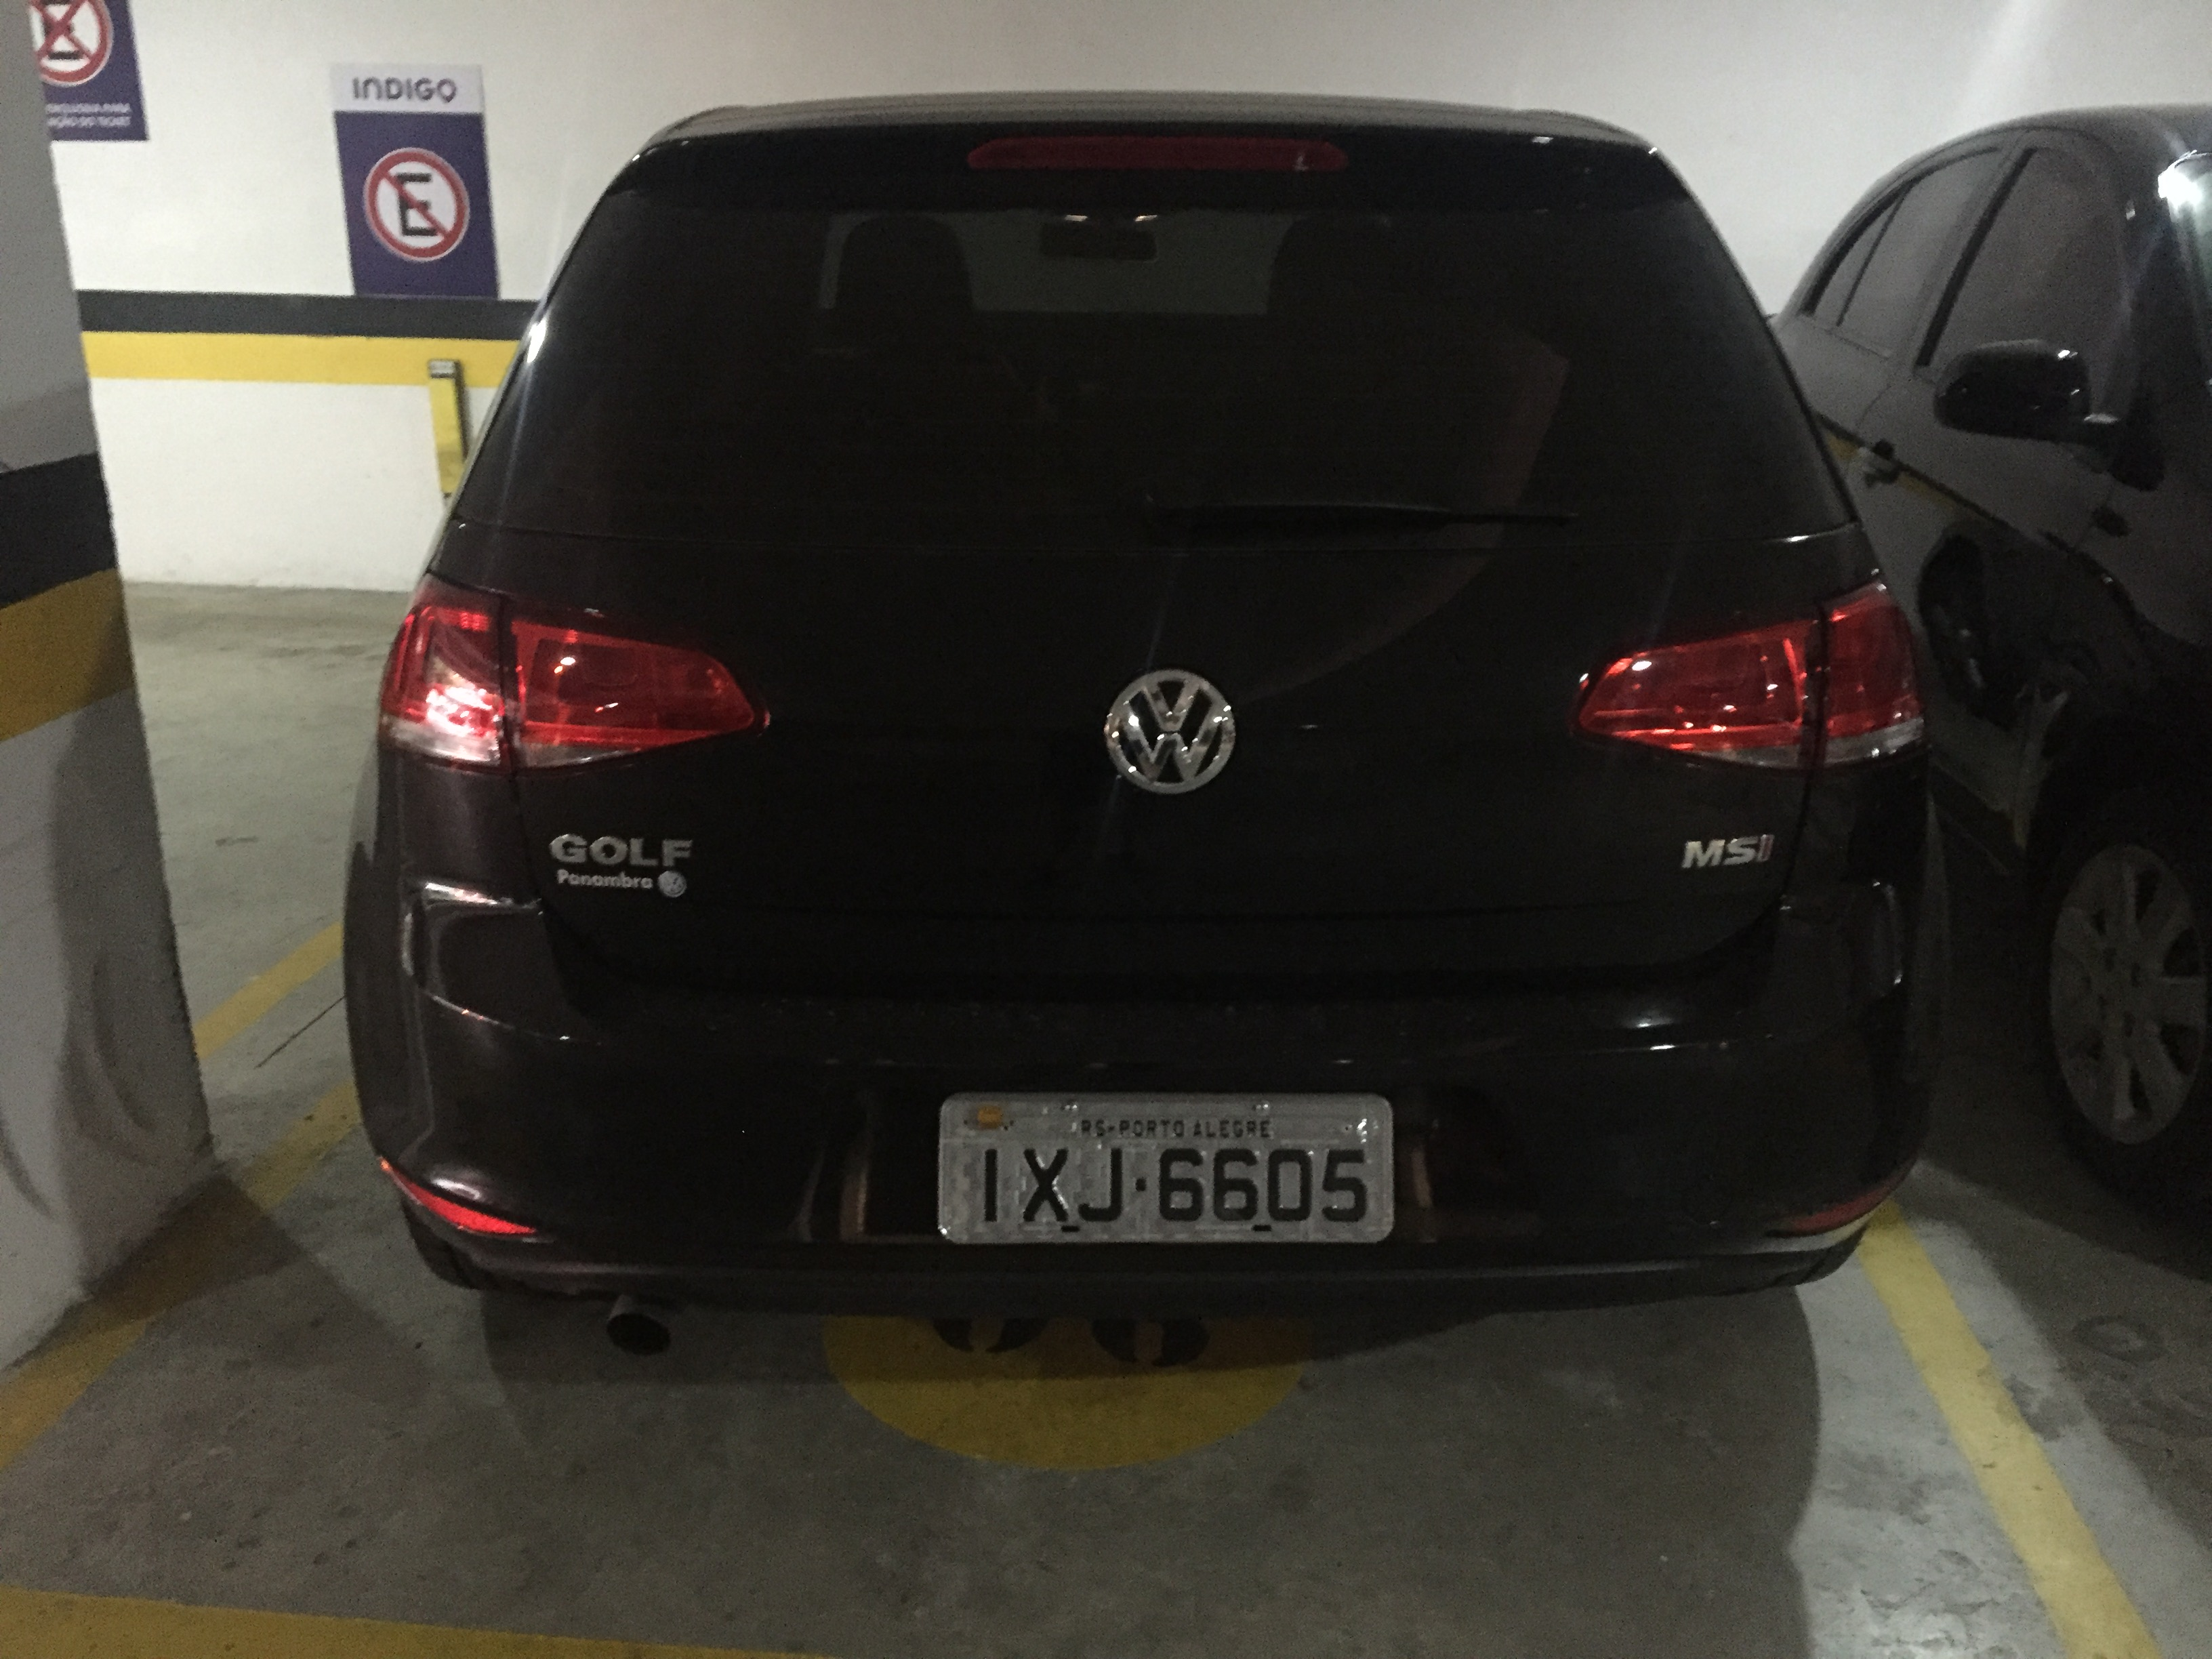
\includegraphics[width=0.70\linewidth]{../../input/full_car.JPG}
	\captionof{figure}{Imagem inicial}
	\label{fig:input_image}
\end{center}

A fase de extração da placa é a fase mais importante em um sistema de reconhecimento de
placas. Todas as etapas subsequentes dependem da exata extração da área da
placa, influenciando o sistema como um todo.

Para a extração das áreas candidatas são utilizadas diversas técnicas de processamento de
imagem em sequência.

\begin{itemize}
	\item Remoção de ruídos e aumento de contrastes.
	\item Detecção de bordas
	\item Preenchimento dos contornos
	\item Abertura e fechamento morfológico
\end{itemize}

\begin{center}
	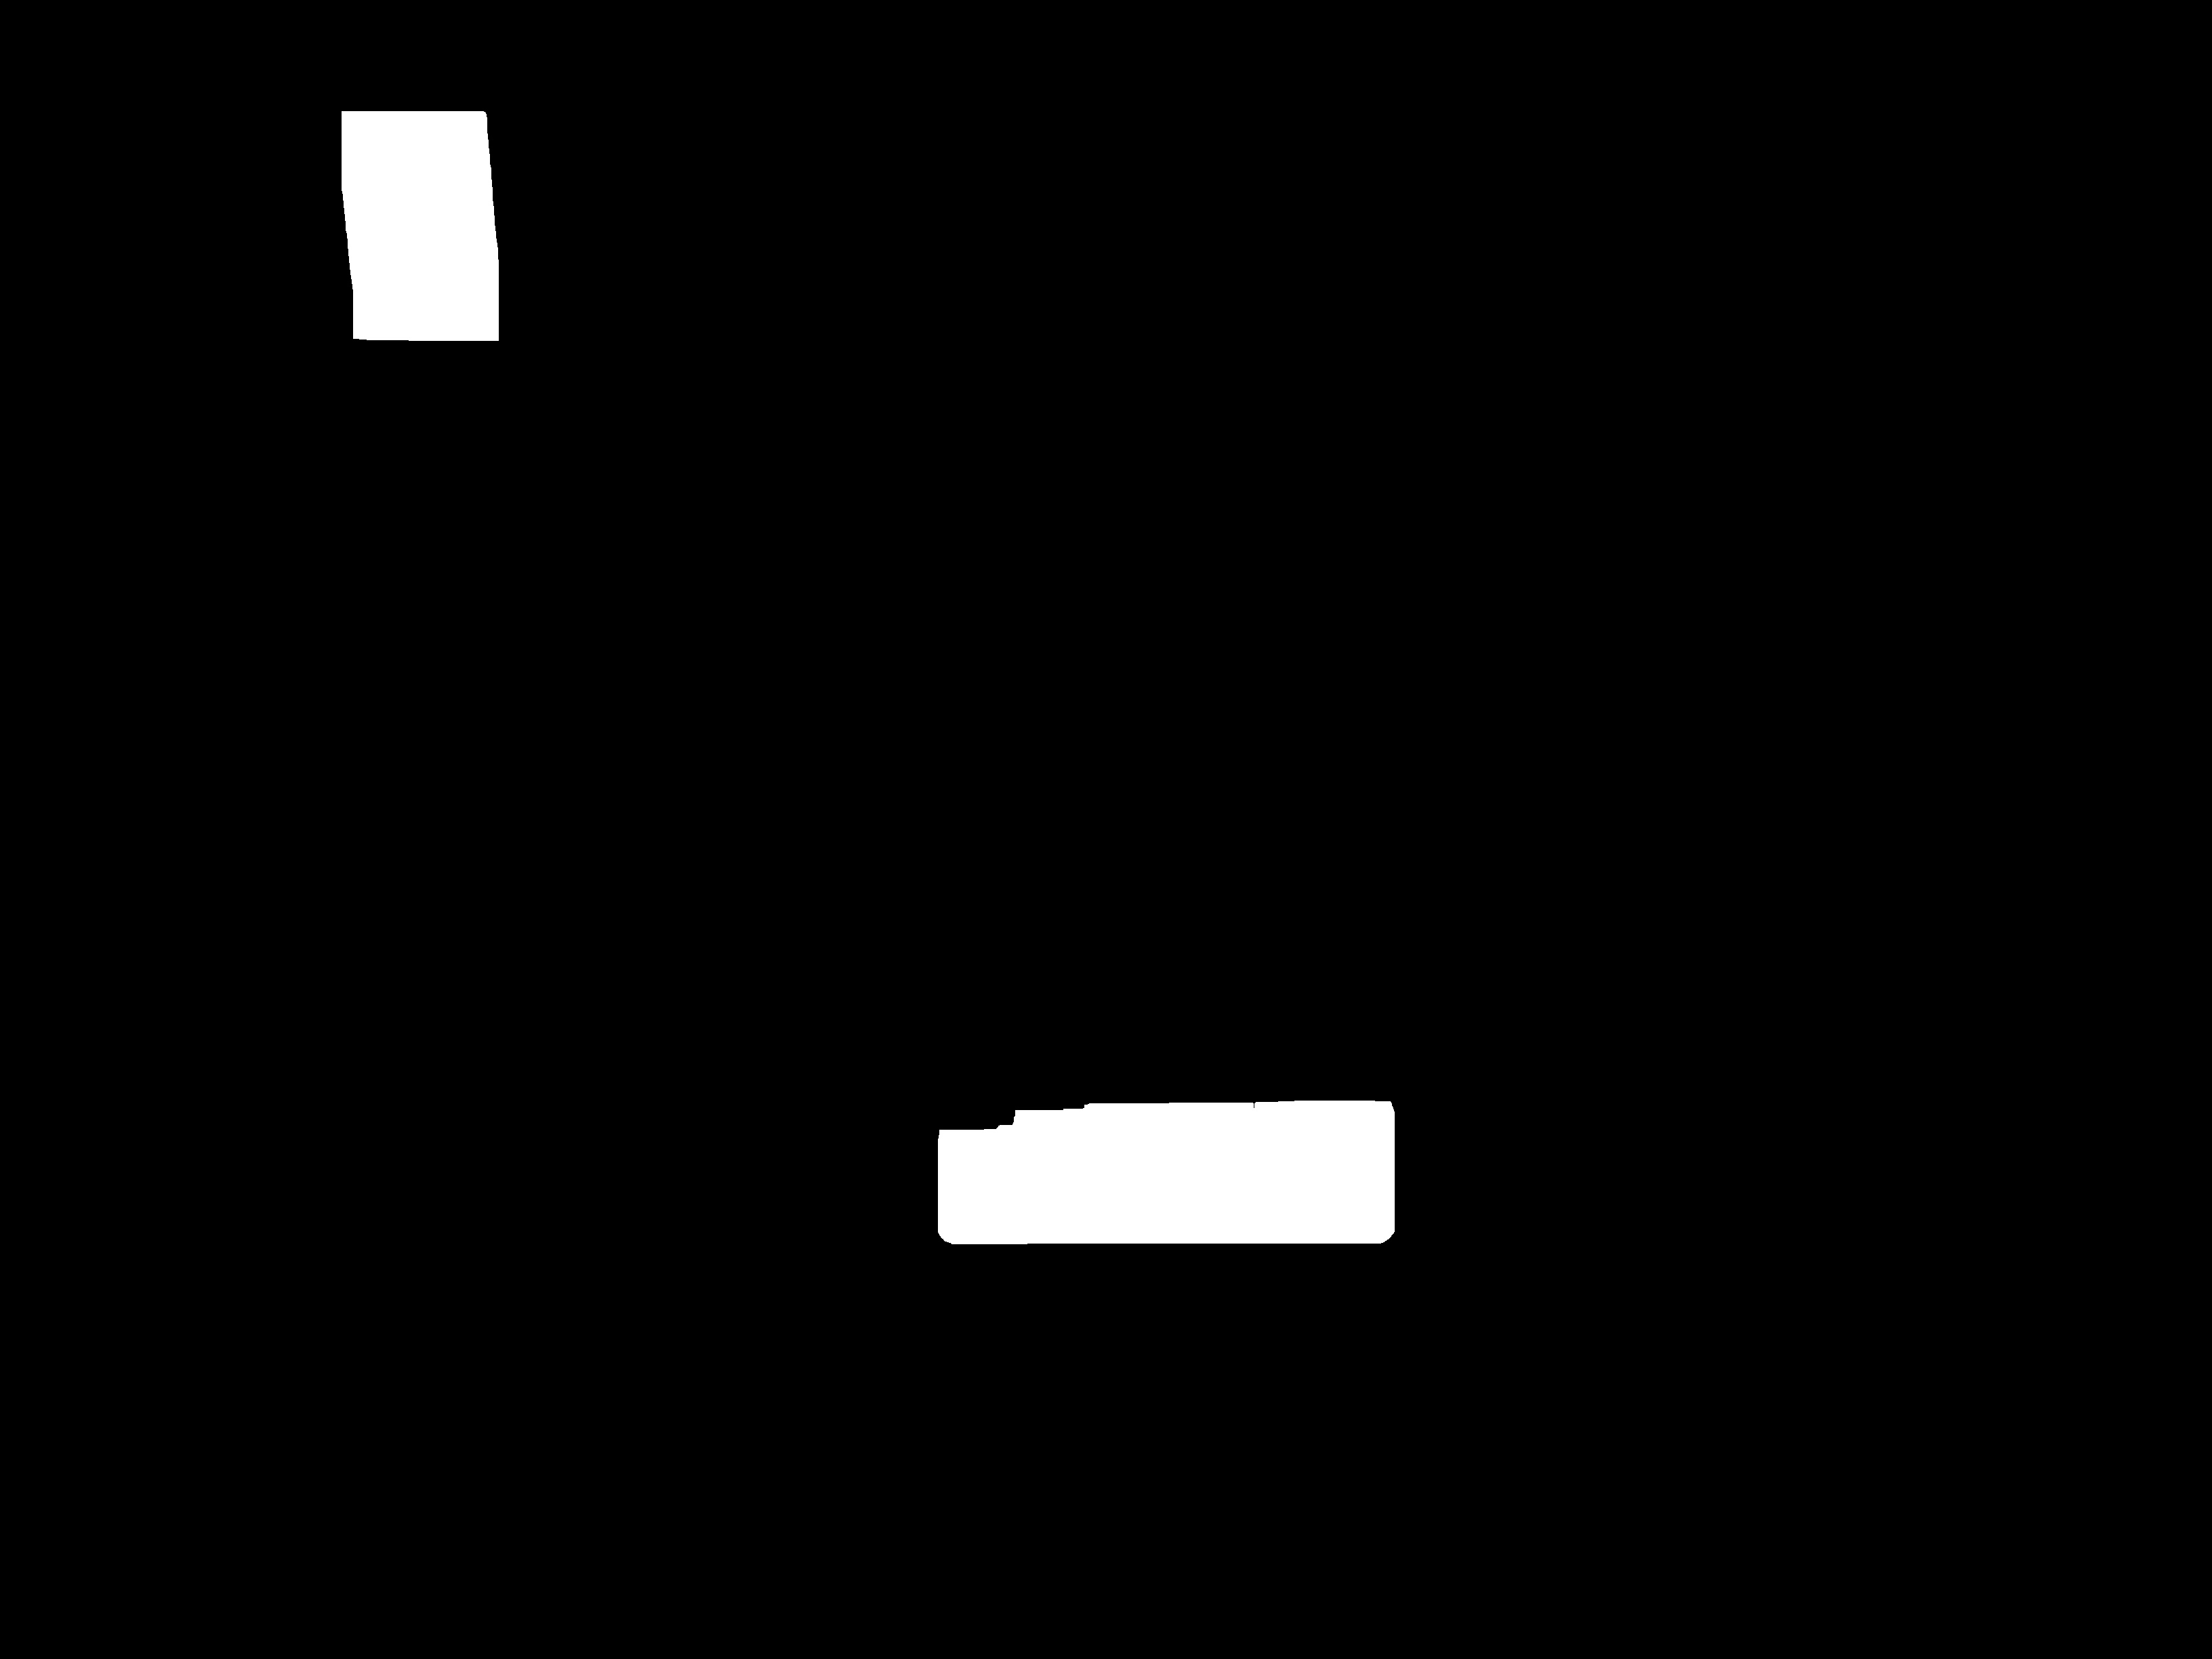
\includegraphics[width=0.70\linewidth]{9fill_dilated.jpg}
	\captionof{figure}{Regiões de Interesse}
	\label{fig:fill_dilated}
\end{center}

Com a região da placa detectada é feita a segmentação dos caracteres. Ela é realizada
com base na conectividade dos pixels. São encontrados conjuntos de pixels conectados na imagem e
se a caixa delimitadora desse conjunto de pixel tiver um tamanho relativo ao tamanho da placa
que a enquadra em um caractere, este espaço é segmentado para ser reconhecido.

\vspace{2cm}

\begin{center}
	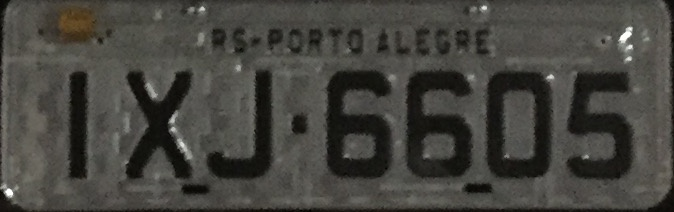
\includegraphics[width=0.70\linewidth]{10roi.jpg}
	\captionof{figure}{Placa Extraída}
	\label{fig:license_plate}
\end{center}

\begin{center}
	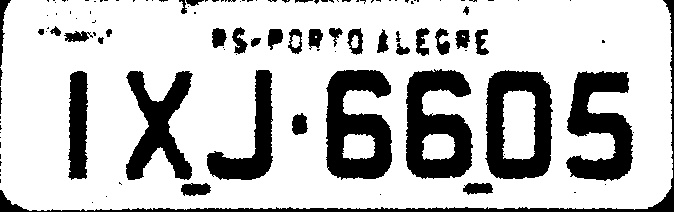
\includegraphics[width=0.70\linewidth]{a02fill_binary.jpg}
	\captionof{figure}{Preparando para o \textbf{OCR}}
	\label{fig:plate_filled}
\end{center}

\begin{center}
	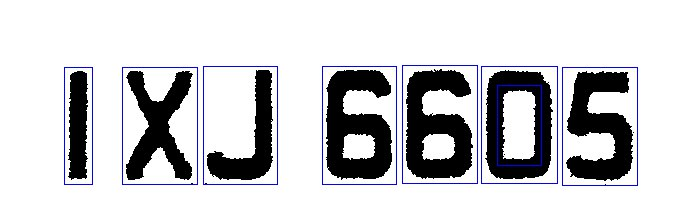
\includegraphics[width=0.70\linewidth]{character_segmentation.jpg}
	\captionof{figure}{Segmentação de Caracteres}
	\label{fig:character_segmentation}
\end{center}

O último passo para reconhecimento da placa é o reconhecimento ótico dos
caracteres extraídos. Para esta etapa foi utilizada uma técnica de \emph{Machine Learning}
de aprendizado supervisionado chamada \emph{K-Nearest Neighbors}.
O modelo é treinado utilizando-se de uma base de dados com todos os caracteres
de A a Z e de 1 a 9 na fonte \emph{Mandatory}, que é a fonte utilizada nas placas de
trânsito brasileiras. O algoritmo funciona posicionando esses dados de treinamento
em um espaço de N dimensões e depois tentando classificar novos dados com bases nos anteriores,
encontrando os pontos mais próximos neste espaço.

\color{NavyBlue}
\section*{\huge Resultados}
\color{Black}

Nas imagens pode-se observar os resultados dos processamentos executados em cada 
passo do algoritmo. A localização da placa na imagem e a segmentação
dos caracteres para reconhecimento.


% ---------------------------------------------------------------
% 	REFERENCES
% ---------------------------------------------------------------
% \vspace{-10mm}
% \large
% \color{NavyBlue}
% \color{Black}
% \raggedright
% \bibliographystyle{plain}
% \bibliography{poster}

\end{multicols}

%----------------------------------------------------------------------------------------
\end{document}
